% Copyright (c) 2014,2016,2018 Casper Ti. Vector
% Public domain.

\chapter{地形编辑器架构设计}
本文的地形编辑器基于ViWo系统的虚拟地球实现,虚拟地球的特点是地形数据量巨大,无法一次性载入内存,用四叉树分层组织数据,绘制时地形数据在内存中动态的换入换出。为了减少从硬盘读取数据的次数,系统中使用LRU算法对地形数据进行缓存,使地形数据可能有多个来源,这增加了数据同步的困难。为此,地形编辑器架构设计的首要目的是调度编辑所需的地形数据,将编辑结果正确的向多个来源、多个层级的地形数据进行同步,并实时显示在分层地形上。其次,地形编辑器可编辑的数据包括地形高程、纹理、语义等,这些数据虽然在数据格式、大小、内容和数据定义细节上有所不同,但形式上都是等宽高的二维数组。因此编辑器设计需考虑数据结构和编辑流程的可扩展性和复用性。本章介绍了系统中分层四叉树的数据管理和调度方式,并据此阐述了地形编辑器架构设计思路,最后对地形高程、纹理和语义编辑的通用流程进行了说明。\par
\section{基于分层四叉树的地形数据管理}                       
分层四叉树的每个子节点是一个地形块,其功能类似于“容器”,用于挂载绘制地形所需的多种数据,包括高程数据、纹理数据、蒙版数据和语义数据等。数据缓存块管理器用于代理地形数据的请求,四叉树向数据缓存块管理器请求地形块数据后,管理器将地形数据载入内存,并将数据以缓存块的形式驻留在缓存队列中。对于已经存在在缓存队列中的块,请求时按LRU算法调整缓存块在缓存队列中的位置以优化数据查找命中率,并将数据指针返回给地形块。地形绘制所需的多种数据的组织和调度方式基本相同,因此对数据缓存块类、数据缓存块管理器类等以模板的形式进行了实现,以便灵活的支持不同类型的地形数据。\par

本系统使用的地形数据块通过其在分层四叉树中的层数$level$、其横坐标$x$和纵坐标$y$进行索引和定位,$x$轴垂直于地球经线,沿经度递增方向递增,$y$轴垂直于地球纬线,沿纬度递增方向递增。每个地形块对应一个唯一的索引,系统中使用地形块进行管理的数据结构都以索引作为关键字进行存储。通过指定在分层四叉树中的层数,以经纬度为$(-180,-90)$的点作为原点,地球上某点的经纬度可以转换为其在数据库中的地形块索引。以经纬度为$(lon,lat)$的某点$k$为例,指定其层数为$level$,其所在地形块$b$的索引为$i_b=(x,y,level)$,有如下关系:
\begin{equation}
\left\{ \begin{aligned}
&originlon=-180\\
&originlat=-90\\
&x=floor((lon-originlon)/(180/(2^{level})))\\
&y=floor((lat-originlat)/(180/(2^{level})))
\end{aligned}\right.
\end{equation}

已知地形块$b$的索引,可快速获知其父子节点索引。$b$与其父节点$p$的索引$i_p$和其子节点$c_1$、$c_2$、$c_3$、$c_4$的索引$i_{c1}$、$i_{c2}$、$i_{c3}$、$i_{c4}$坐标存在如下关系:
\begin{equation}
i_p = (x/2,y/2,level-1)
\end{equation}
\begin{equation}
i_c = \left\{ \begin{aligned}
&(x*2,y*2,level+1)\\
&(x*2+1,y*2,level+1)\\
&(x*2,y*2+1,level+1)\\
&(x*2+1,y*2+1,level+1)
\end{aligned} \right.
\end{equation}
分层四叉树地形绘制的基本流程为(1)遍历四叉树,找到所有符合精度要求的覆盖地形的四叉树节点;(2)根据视口对节点进行剪裁;(3)获取待绘制节点的数据;(4)向GPU打包发送数据;(5)在GPU绘制。在虚拟地球的使用场景中用户视角是不断变化的,因此基于以上所示父子节点的关系,在视角运动的过程中,每一帧都重新自顶向下的构造分层四叉树。构造时遍历四叉树的子树,若节点精度不满足当前视角所需的分辨率,地形块会分裂为四个子块,即继续检查该节点的四个子节点。直到子节点的数据精度满足某个阈值,则停止分裂,并向数据缓存块管理器请求这些子节点的数据。\par
数据请求发生时,数据缓存块管理器首先从LRU缓存队列中查找地形块缓存,如果存在,则将缓存块的指针赋给地形块节点使用,如果不存在,则发起从本地获取地形块数据的请求。地形高程和纹理数据在本地以BerkeleyDb\supercite{Db}的数据库格式存储,数据缓存块管理器以地形块索引作为关键字向数据库请求地形块数据。由于涉及大量计算、查找和数据传输操作,同步的从本地数据库请求数据的时间效率不能满足实时漫游的流畅性需求。系统中实现了线程池和任务队列来管理地形块请求任务,将地形块数据请求作为一个任务添加到任务队列中异步的处理。使用多线程进行数据加载可以使界面交互不会被数据请求阻塞。自顶向下异步的请求地形块可以保证绘制的连续性,视口中的画面可能经历从粗糙到精细的加载过程,当这个过程非常短时对视觉效果影响较小。
\par

\section{基于规则网格的实时编辑}
对基于规则网格的地形进行笔刷编辑时,需要考虑笔迹的形成方式、在内存中的表示方式、笔刷的性质(如形状、直径、硬度等)以及笔迹对网格数据的编辑算法等问题。比起在单层地形上编辑,在分层四叉树上编辑的地形编辑器有诸多难点,包括编辑时笔迹所经过的地形块可能跨越多个层级、编辑结束后编辑结果向地形金字塔上层和下层的同步、首次从数据库中载入地形块后现有编辑结果向新载入块的同步,以及编辑结果在分层地形上的实时呈现等等。在分层地形编辑器中实现笔刷编辑需要对以上问题进行设计,兼顾鲁棒性和时空效率。\par
\subsection{编辑器架构}
地形模块是ViWo系统的核心模块,地形编辑器则以插件的形式,独立于地形模块存在。地形模块对地形数据的操作主要为获取地形数据、缓存地形数据、用地形高程和纹理数据进行绘制,同时其他模块还会通过地形模块提供的接口获取语义数据。地形编辑器在设计时需要将地形编辑逻辑与地形模块基本流程进行拆分,不启用地形编辑器插件时基础地形模块的绘制效率和运行流程不受影响。为此,在地形模块定义基类,实现地形绘制所需的基本功能,并在编辑器模块对基类进行派生,以多态的形式使地形模块支持编辑功能。如图3.1所示,红框表示基础地形模块所包含的主要功能,蓝框表示地形编辑器所包含的主要功能。加载地形编辑器插件时,用派生类对象替换基类对象,将地形编辑功能注入到基础地形流程中。\par

\begin{figure}[htbp]
\centering
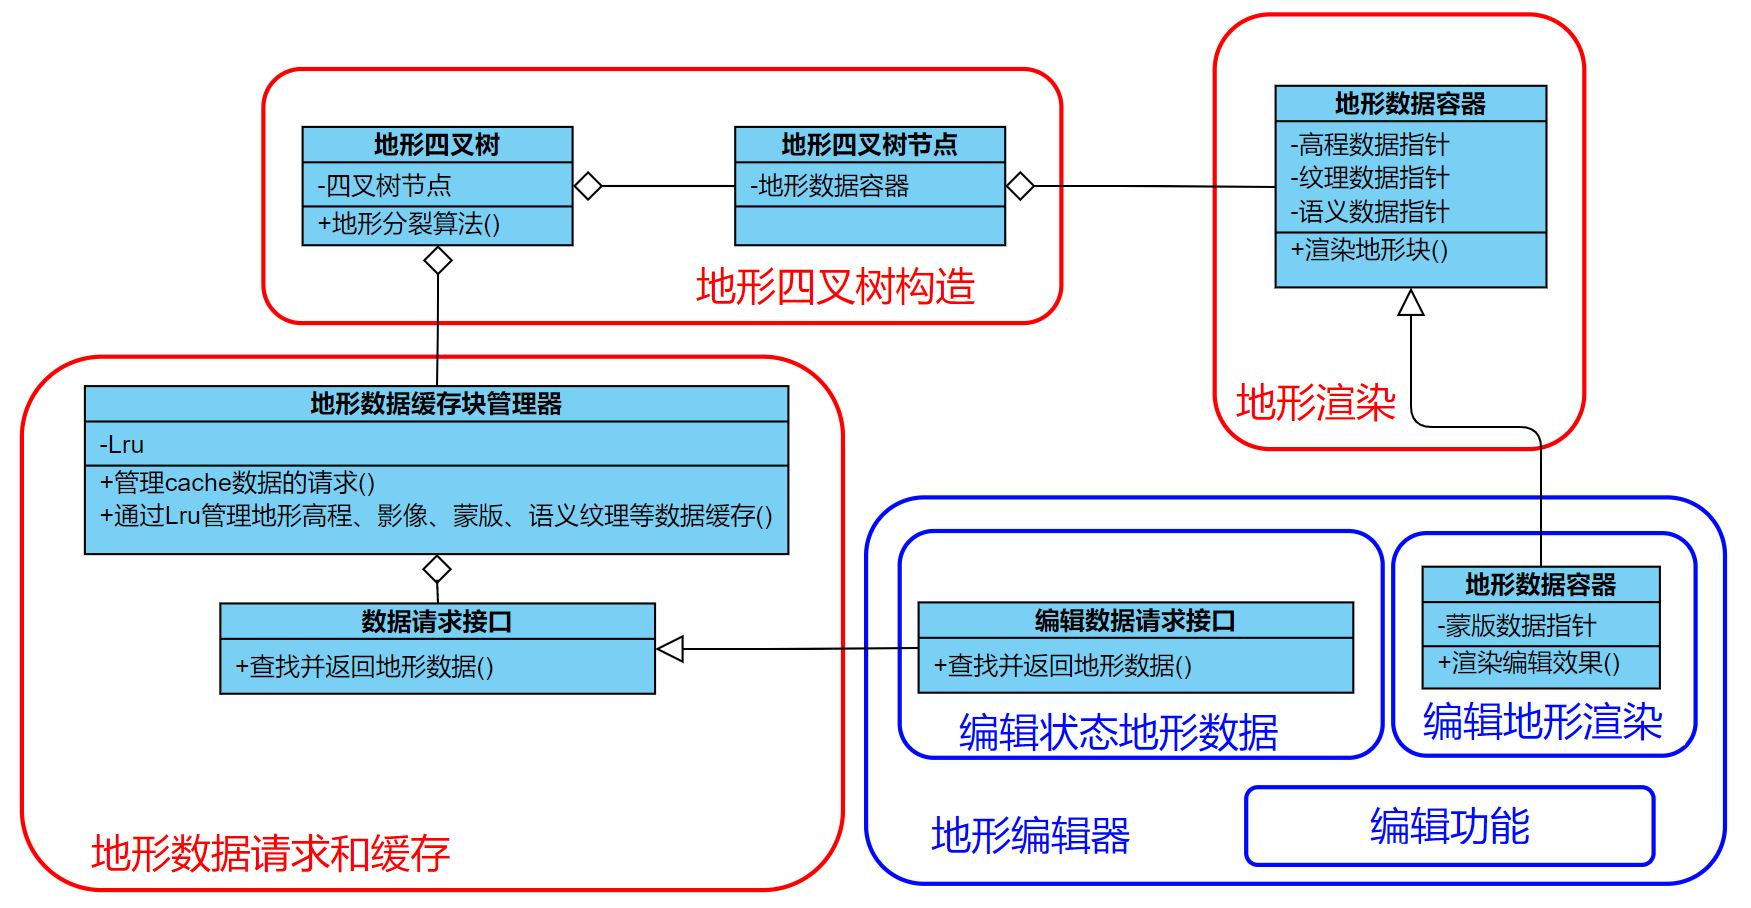
\includegraphics[height=7cm,width=13.2cm]{figures/editorStructure.JPG}
\caption{地形及编辑器功能模块图}
\end{figure}
本系统中用过滤\supercite{summer}来定义将编辑操作应用到高程数据上的过程,并定义过滤器为保存多次编辑操作的容器。编辑模式下请求地形数据时会经过过滤器,并检查当前地形数据上是否应用了所有编辑操作。考虑到使分层四叉树处于可编辑状态会带来额外的时间、空间开销,因此即便在配置文件中设置了加载编辑插件,也只在用户通过点击按钮开启高程和纹理编辑工具时,才替换基础地形数据结构为编辑状态的地形数据结构。由于分层四叉树每帧都重新构造,地形块内的数据也在四叉树构造时重新请求并挂载,因此在重新构造四叉树的过程中,可以自然的完成从普通状态地形块到编辑状态地形块的替换。实现中,在地形块内保存地形状态,在构造分层四叉树时通过检查当前地形状态是否与地形块内保存的地形状态相符。若不相符,则向地形块构造器重新申请地形块,并通过编辑模块派生的地形块构造器,构造具有编辑功能的地形块数据结构。对于数据缓存块管理器,不能用其派生类直接替换。因为LRU缓存队列包含了已经加载进内存的地形数据,重置数据缓存块管理器将导致现有的LRU缓存队列失效,并重新加载地形。因此不对数据块缓存管理器类进行派生,而是将其中数据请求相关的函数抽出作为一个类,对该类进行派生。
\subsection{编辑数据结构定义}
以油画绘制对地形的笔刷绘制做类比,可以认为一幅画是由若干笔迹构成的。产生笔迹的途径是使用画笔在画布上产生连续的若干个点,绘画者通过选择笔刷掌握笔迹的颜色、粗细、纹理、力度等特性。画布承载了画笔的若干条绘制结果,笔迹之间存在先后关系,从下到上按笔迹产生的顺序依次叠加在画布上。本系统中实现了笔刷、编辑曲线绘制工具、补丁数据等类,与笔头、画笔、局部画布等概念进行映射,下面对这些类一一进行阐述,并由图3.2阐述了类之间的关系。\par
\begin{figure}[htb]
\centering
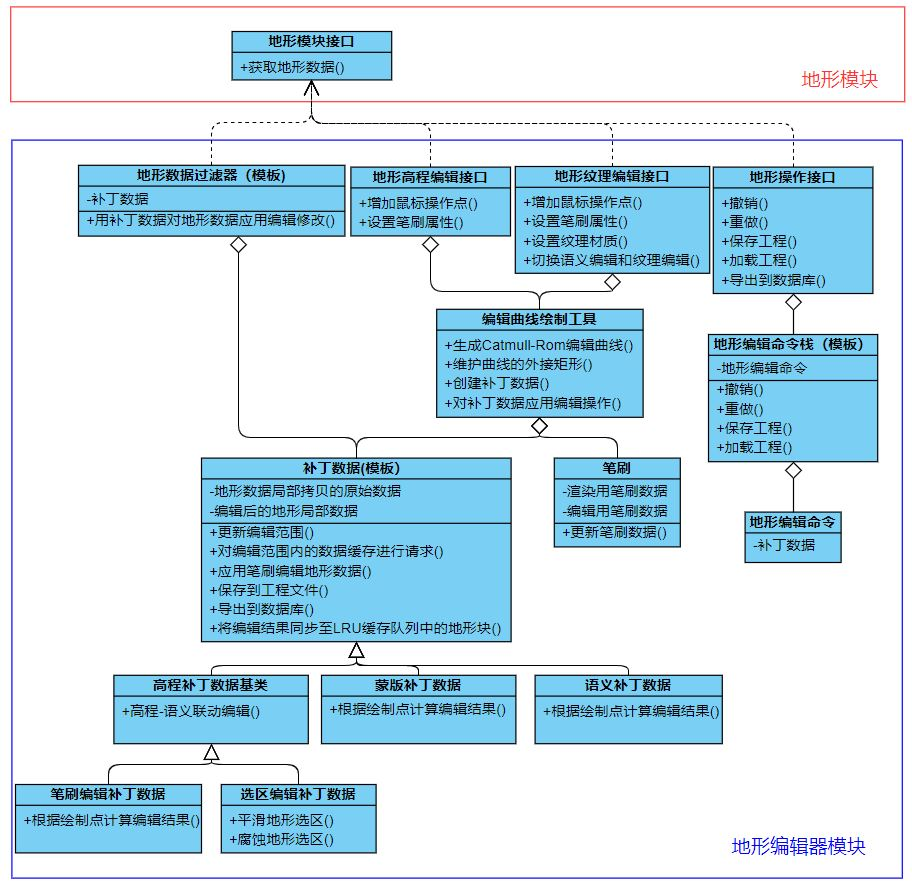
\includegraphics[height=12.8cm,width=12.5cm]{figures/structure2.JPG}
\caption{地形编辑器架构中核心类关系图}
\end{figure}
\paragraph{笔刷类}
高程编辑改变的是地形网格的高程数据,由测绘产生的地形高程数据本身分辨率不够高,网格不够密,因此更需要保持数据的连贯性,使编辑后的区域与未编辑区域可以平滑过渡。而地形纹理编辑的编辑结果需要有一定的随机性,看起来才更加自然。因此编辑器为高程和纹理编辑分别提供了两种笔刷,高程编辑为圆形笔刷,编辑强度从笔刷中心向笔刷边缘平滑降低。纹理编辑的笔刷以多种形状的笔刷模板的形式提供,编辑时笔刷模板中的每个数据与地表纹理中的数据一一对应,并指导在该像素处的颜色混合。
\paragraph{编辑曲线绘制工具类}
在本系统中,一次编辑操作定义为,一次鼠标按下拖拽并抬起的过程中,由若干离散鼠标采样点连成折线构成的单条笔迹。编辑曲线绘制工具的功能类似画笔,主要实现了将若干采样点转换为一条Catmull-Rom曲线,并控制具有大小、硬度等属性的笔刷在“画布”上进行修改的功能。Catmull-Rom样条曲线的一个特性是曲线经过所有控制点\supercite{catmull-rom},用离散采样点构造的Catmull-Rom曲线可以很好的拟合鼠标连续拖动形成的编辑笔迹。编辑曲线绘制工具从高程编辑接口接受鼠标轨迹采样点,构造Catmull-Rom曲线。鼠标点的采样频率与实时帧率相关,鼠标快速滑动或帧率发生波动时,两个采样点中间可能间距过大导致笔迹曲线不平滑。因此在两个采样点中间插入Catmull-Rom曲线上的点,插入的点称之为参考点。计算采样点之间的距离,使两个采样点间参考点的数目基本与距离成正比,使笔迹曲线样条形状更有一贯性,更加平滑。所有采样点和参考点统一作为绘制点参与笔迹绘制。目前笔刷的可调参数包括笔刷的直径和硬度,在此基础上,高程笔刷形状为圆形,纹理笔刷可以选择形状和编辑规则。在编辑曲线绘制工具的层面,对于高程和纹理编辑的笔刷编辑来说,增加笔迹点和生成笔迹曲线的逻辑是相同的,但在使用笔迹曲线对补丁数据进行修改的具体实现中,高程、纹理和语义编辑存在一定区别,分别在补丁数据的层面进行了实现,在本文后面的章节会进行详述。\par
\paragraph{补丁数据类}
编辑操作所保存的数据结构称为补丁数据,补丁数据是一块或多块相邻地形块高程或纹理数据的完整拷贝,可以看作“从画布上复制了画布的一块局部”。考虑一笔笔迹内所涉及的地形块在绘制时可能处于不同层,因此每开始一条笔迹时,即向编辑曲线生成工具添加笔迹的起始点时,生成一块新的画布。这块画布是现有地形的一个局部,包含之前所有的编辑结果。规定生成补丁数据时,拷贝原始数据的层级为当前分层四叉树中最精细层。笔迹的外接矩形表示了本次编辑的范围,此矩形与最精细层级的若干地形块相交,这些地形块的数据是直接参与本次编辑的,编辑前首先将其按原有空间位置关系拷贝到补丁数据中。编辑时对数据的修改首先应用到补丁数据上,并在编辑结束后,由补丁数据向LRU缓存队列中所有与补丁数据有交的块分发,即“将局部画布贴回画布上,覆盖画布中原有的内容”。如图3.3所示,某个局部区域中相邻的四个地形块上的编辑结果由三次操作产生的三个补丁数据按顺序叠加而成,可以看到第二个和第三个补丁数据上包含了之前的编辑结果。\par

\begin{figure}[htbp]
\centering
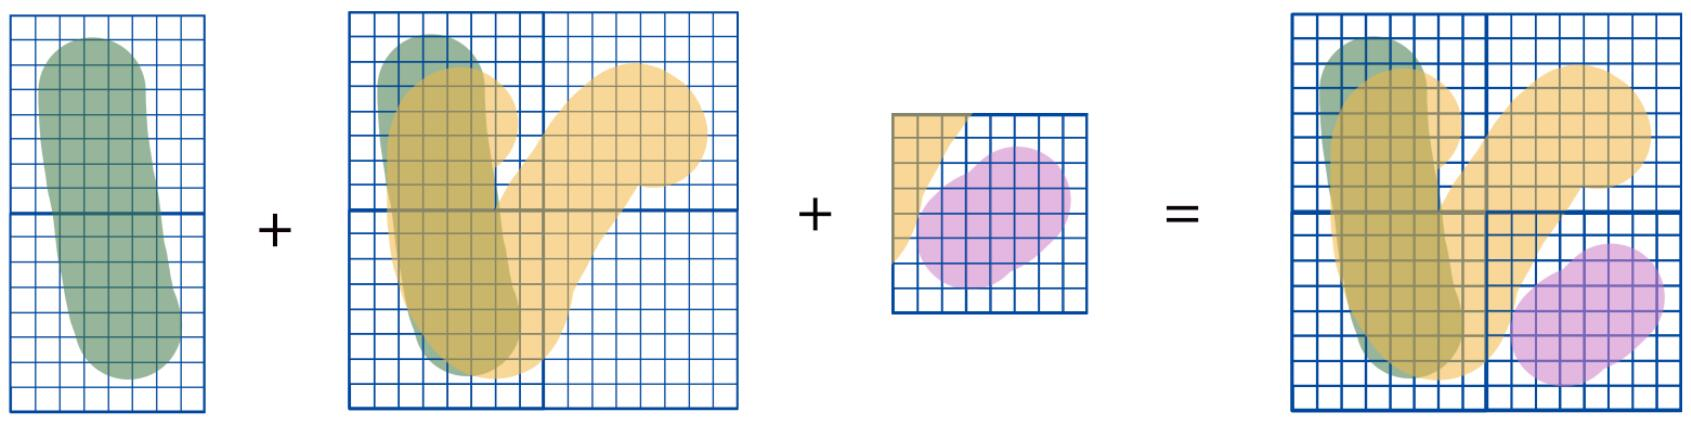
\includegraphics[height=3.9cm,width=14.8cm]{figures/mergeData.jpg}
\caption{补丁数据叠加作用形成最终的数据}
\end{figure}

\subsection{基于笔刷的实时编辑流程}
图3.4示意了笔刷实时编辑时编辑器的大致工作流程,流程的输入为若干个鼠标位置点,输出为一个编辑完的补丁数据,用补丁数据将修改结果分发到各个地形缓存块中后流程结束。\par
\begin{figure}[htbp]
\centering
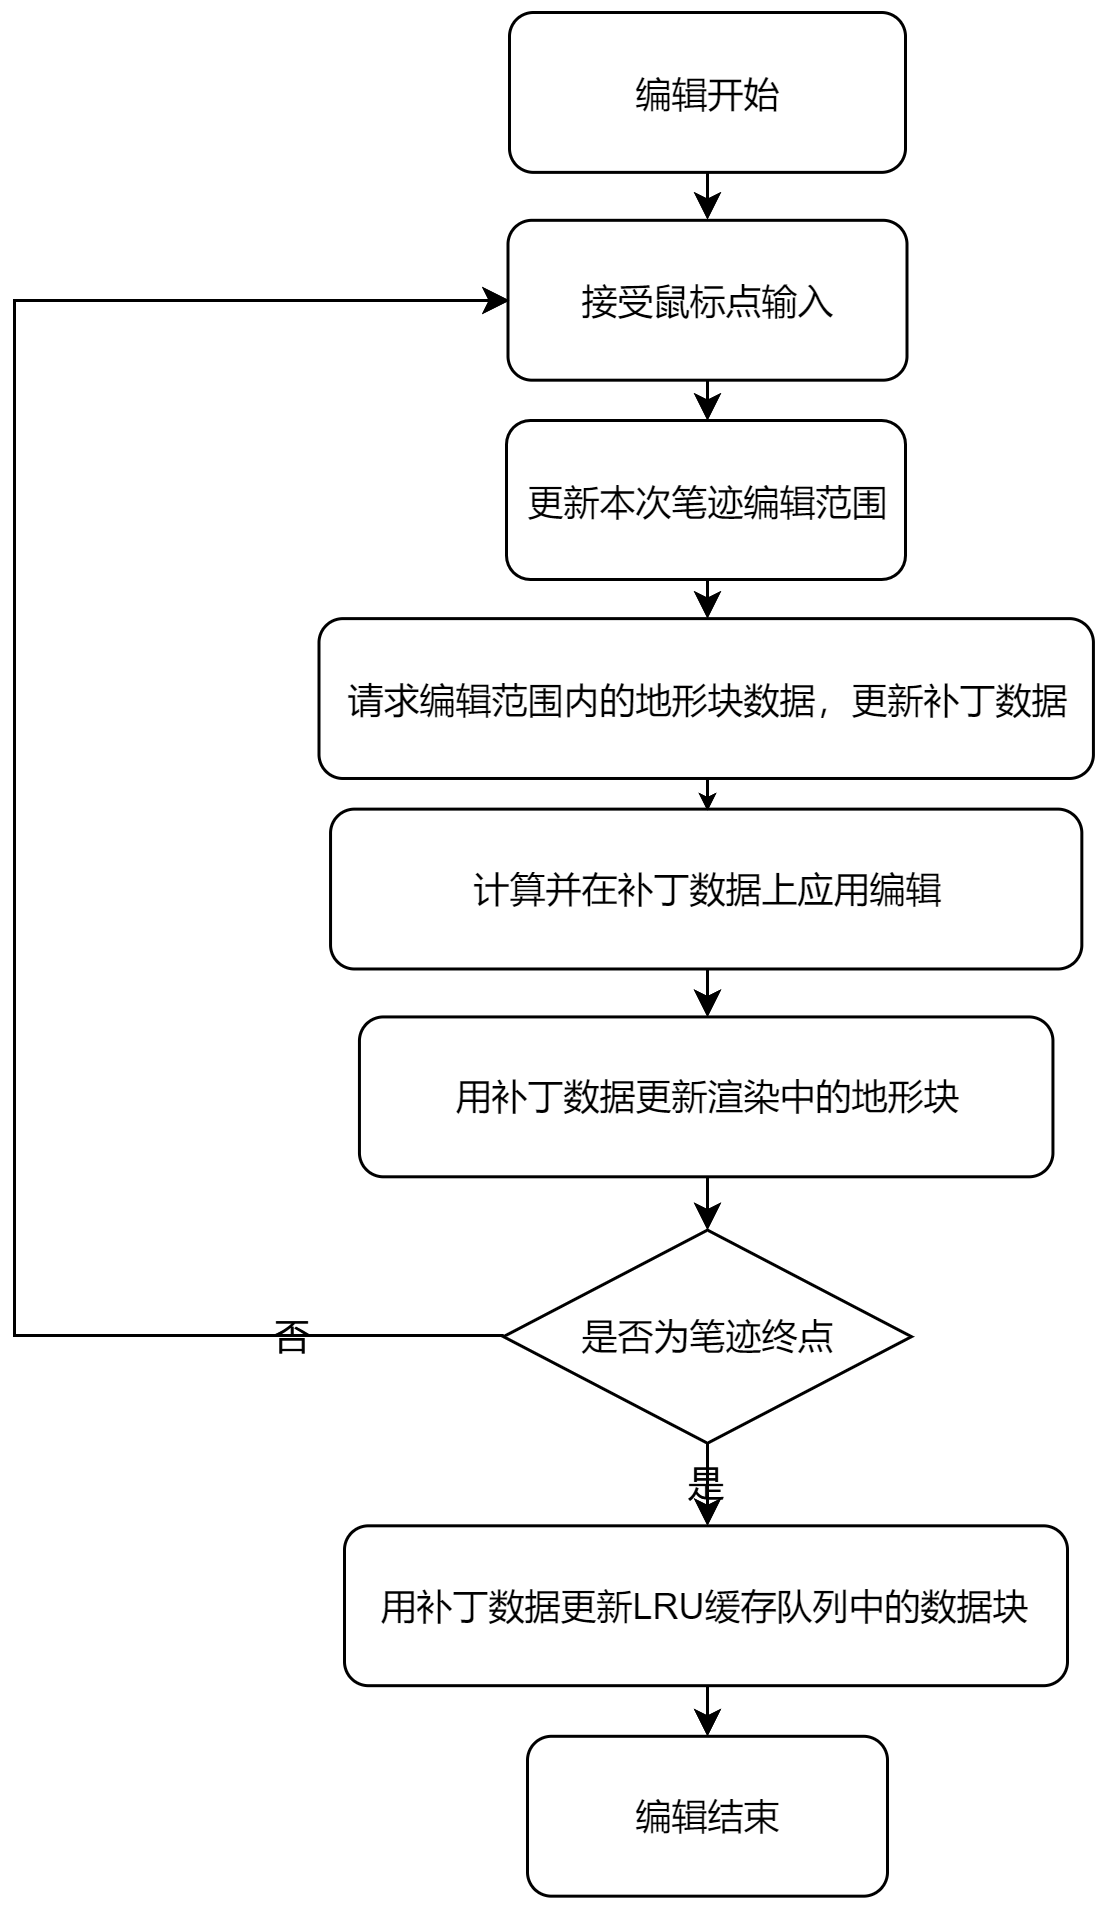
\includegraphics[height=11.6cm,width=6.5cm]{figures/flowChart.png}
\caption{笔刷实时编辑流程}
\end{figure}
一次编辑开始后,编辑曲线绘制工具根据当前分层四叉树的最精细层级创建一块初始的补丁数据,并清空上一次编辑的曲线数据,开始维护本次的编辑曲线数据。每向曲线中插入一个点,都会导致一次编辑范围的更新。图3.5展示了鼠标由位置\circled{1}拖向位置\circled{2},产生两个鼠标采样点的过程。平铺的蓝框表示若干地形块,其层级为当前分层四叉树中最精细的层级。红色和蓝色的同心圆分别表示笔刷的内直径和外直径,黄色和红色的虚线框和区域分别表示第一次和第二次更新编辑范围后,两个笔刷绘制点的外接矩形,及外接矩形与地形块求交得到的编辑范围。因此编辑范围发生变化时,为补丁数据重新分配内存,并对编辑范围内的地形块数据发起请求,拷贝原始数据填充补丁数据。\par
\begin{figure}[htbp]
\centering
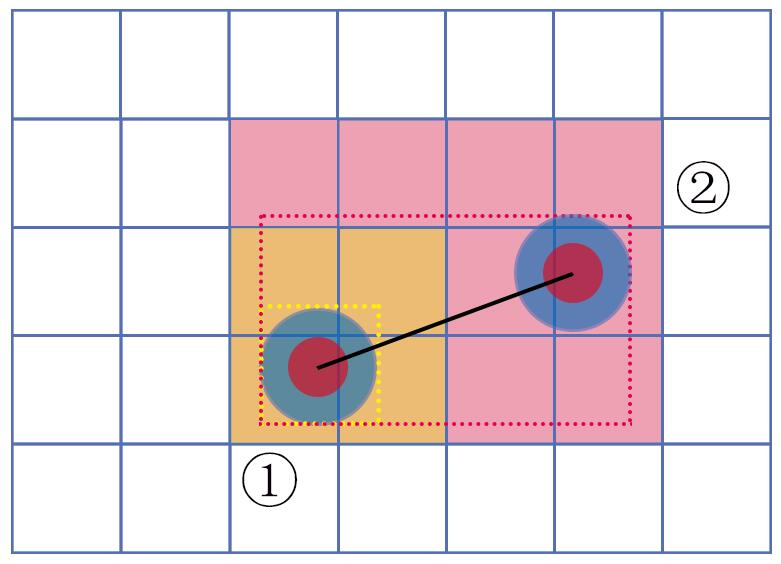
\includegraphics[height=4.3cm,width=6.2cm]{figures/brushRange.jpg}
\caption{编辑范围更新}
\end{figure}
称编辑时确定待编辑像素范围和数据变化情况的算法为笔刷编辑算法,高程编辑和纹理编辑分别对笔刷编辑算法进行了不同的实现,分别在第四、五章进行了阐述。\par
编辑结果从补丁数据向地形块数据的分发有两个阶段。第一个阶段是每接受一个鼠标采样点并对补丁数据进行修改后,将最新的编辑结果分发至补丁数据所覆盖的绘制中的地形块。这一阶段分发的目的是在用户拖动鼠标时实时的呈现编辑效果。第二个阶段是整条笔迹结束后,将保存了完整编辑结果的补丁数据,分发至地形金字塔所有层次中与该补丁数据有交且缓存在LRU队列中的地形块。这一阶段分发的目的是为了使编辑结果在地形金字塔的所有层次中同步。在第一阶段的分发中,由于补丁数据拷贝了最精细层级的数据,但处于绘制状态中的块并不都是最精细层级的块,可能是最精细层级的父块。因此对于补丁数据所覆盖的最精细层级块,如果当前绘制的并非该块而是其父块,则设置其父块为该块的关联块,并在第一阶段分发时分发到其关联块,以保证编辑结果的实时呈现。\par

补丁数据是保存了编辑结果的关键数据,应当能重复应用,使编辑结束后才请求到内存中的地形块也能正确的呈现编辑结果。因此,补丁数据创建后主动将自己注册到过滤器中保存。为了区分不同来源的数据块对编辑操作的应用情况,为数据块添加一个属性表示已经经过了多少次编辑操作。当对数据块进行过滤时,只对超出当前编辑次数的编辑操作进行应用即可。如本章上面内容所说,地形数据可能存在的位置有两种,一种是保存在本地数据库中的原始数据,另一种是绘制时被请求到内存中,并在LRU缓存队列中进行缓存的数据,发生数据请求时首先从LRU的缓存队列中查找块。过滤操作可以保证不同来源的地形数据都应用相同的编辑。对于LRU缓存队列中的地形块,编辑结束后立即应用编辑操作,使分层四叉树可以获得最新的地形数据。对于未在LRU缓存队列中的地形数据块,当分层四叉树从本地数据请求时,首先经过过滤器,将过滤器中的补丁数据依次应用到新请求的地形块上。\par

\section{编辑器常用功能实现}
对于编辑器来说,除了提供针对具体数据的编辑功能,还需要提供一些编辑器常规功能。在文件层面,对编辑结果进行文件存储和加载等操作,是使编辑成果可以保存和传输的必要功能。在操作层面,增加对编辑操作进行撤销和重做的功能可以提高编辑器的可用性和易用性。

\subsection{编辑操作撤销和重做}
本文基于设计模式中的命令模式,为高程编辑操作提供了撤销和重做功能。通过保存操作命令及其产生的核心数据,可以将操作命令队列保存至工程文件以保存编辑现场。命令模式是常用的行为型设计模式,其主要思想是将操作或命令视作一个对象来保存,并为命令类提供执行、撤销、重做等接口,从而灵活安排执行命令的对象和执行的时刻,降低系统的耦合度。通过正确的定义命令类的数据结构,保存执行命令所必需的信息,持有命令的对象可以复现该命令。\par
产生编辑结果的核心数据是笔刷的属性以及笔迹采样点,通过将这些数据传递给编辑曲线绘制工具,可以产生相同的编辑结果,但由于地形高程数据参与最终结果的插值,因此无法通过简单地将编辑高度设为相反数并应用原笔迹数据来撤销。编辑操作生成的补丁数据保存了当次操作前后局部地形的数据,因此编辑命令保存了补丁数据的指针。撤销时对补丁数据中指向原始数据和修改后数据的指针进行交换,并将原始补丁数据应用到当前地形上。即将补丁数据的编辑范围与LRU缓存队列中地形块进行求交,更新与之有交集的地形块数据。\par
使用双栈保存撤销和重做的操作命令以实现命令的管理和保存功能。一个栈存储命令,称为DoList,另一个栈存储回退了的命令,称为UndoList。命令对象包含一个编号属性,记录命令的发生次序。为保证编辑操作是单线性的,每次有新的操作进入DoList时,清空UndoList。图3.6以标号表示操作的次序,3.6(a)示意了执行操作、撤销和重做命令时,管理命令的双栈中数据发生的变化,图3.6(b)、3.6(c)共同展示了一个撤销操作的实例。如图3.6(b)所示,数字代表一个操作命令,由小到大表示编辑发生的次序,黑色数字表示现在应用的编辑,灰色数字表示回退了的编辑,为保证操作历史的单线性,当6号操作出现时,就需清空UndoList,栈内数据的变动如图3.6(c)所示。\begin{figure}[htbp]
    \centering
    \subcaptionbox{}{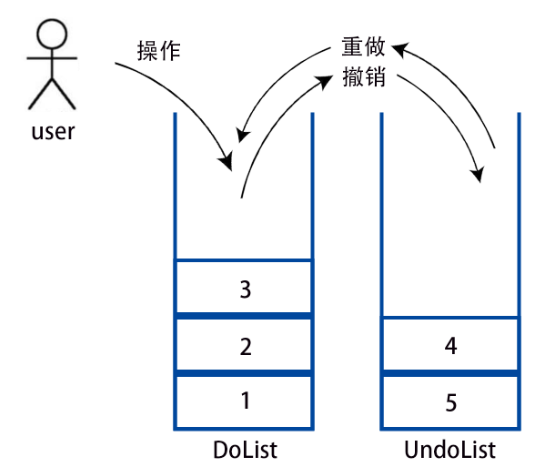
\includegraphics[height=5cm,width=5.8cm]{figures/command.png}}
    \subcaptionbox{}{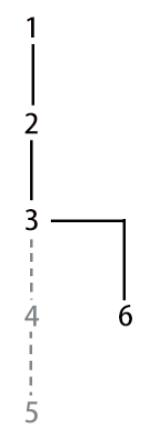
\includegraphics[height=5cm,width=1.5cm]{figures/command3.jpg}}
    \subcaptionbox{}{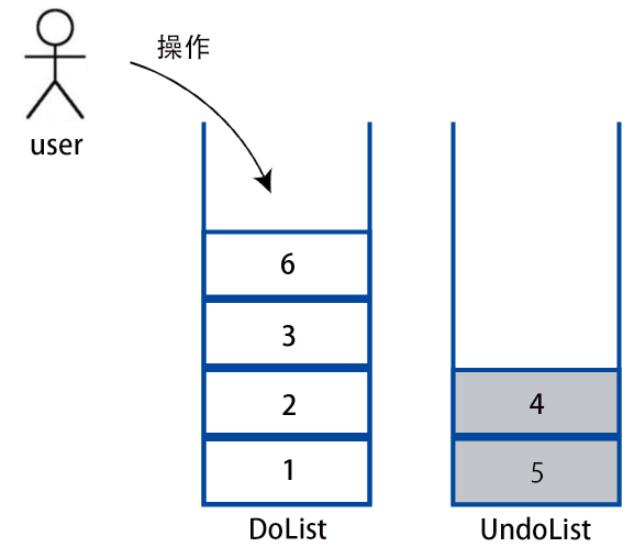
\includegraphics[height=5cm,width=5.8cm]{figures/command2.jpg}}

    \caption{以DoList和UndoList表示存储操作和存储回退的操作的两个栈:(a).操作、撤销和重做时命令对象在两个栈中的流动方向(b).撤销后未进行重做而进行了新的编辑的情况(c).如图(b)所示的情况需要清空UndoList以避免与编辑历史发生冲突}%The experimental results for $R_t= \exp \left( \left[1, -0.5, -2\right]^T \right)$.
\end{figure}
考虑到一个场景的编辑可能涉及上千条笔迹,因此为命令栈设置容量上限,只有容量上限范围内的命令可以撤销和重做,超出容量上限的命令数据可以进行合并优化。
\subsection{工程文件保存和结果导出}
编辑结束后,其结果需要以某种形式进行保存。目前要在系统中漫游精细地形需要配置的地形数据包括地形高程和纹理的两个数据库,为不使配置的复杂度增加,地形高程和纹理的编辑结果可以在导出时并入原数据库或输出到新数据库,用户可以通过配置数据库链式请求的顺序以应用编辑结果。同时,为了方便用户进行二次编辑,类似其他商用设计类软件的,应当提供一种工程文件保留编辑过程。因此分别实现了这两种保存方式。\par
对于写入数据库的保存,首先遍历过滤器,计算分层四叉树所有层级上需要保存的地形块索引,然后请求这些地形块,应用编辑操作后以原分辨率覆写到目标数据库中。以这种方法纹理编辑结果存储存在一定的弊端,一是保存前需要将纹理编辑所有图层的结果计算并叠加在一起,保存过程耗时较长;二是将纹理编辑结果的分辨率固定为与卫星影像源数据相同,分辨率下降,失去了纹理编辑产生的结果比卫星影像更精细的优点。\par
保存工程文件可以在一定程度上弥补写入数据库保存的不足。对于高程编辑操作的保存,命令队列中包含了开始编辑以来对地形高程执行的所有操作,因此对高程编辑操作的保存和加载就是对命令队列的存储和复原。实现中,分别保存Dolist和UndoList中的补丁数据,按顺序以二进制格式写入到本地文件中,需要保存的数据包括补丁数据的宽高、起止点等属性和地形数据本身。加载时,从文件中读取数据生成补丁数据,插入Dolist或UndoList,并注册到过滤器,用补丁数据进行过滤操作,使地形与之前编辑的结果相同。因此,当用户再次编辑时可以通过加载原始的数据库和工程文件恢复之前的编辑现场。对于纹理编辑操作的保存,需要按顺序保存每个图层的信息,包括图层名和图层所使用的纹理数据,以保证加载工程时可以还原图层的编辑状态,且无需在默认纹理库路径下配置之前使用的纹理材质。\par


\section{本章小结}
本章就分层地形编辑器架构设计中存在的一些难点进行了说明,并基于对这些问题的考虑,阐述了ViWo系统中地形编辑器的架构设计,介绍了该架构下实时大规模地形笔刷编辑,编辑操作的撤销和重做,地形编辑结果保存和加载等功能的实现方法。该架构还考虑了可扩展性,能应用在多种基于规则网格的数据的编辑上。下面两章将分别介绍高程和纹理编辑的实现细节和不同之处。
% vim:ts=4:sw=4
